\newcommand{\dd}{\mathrm{d}}

Začneme náš kurz jakýmsi rychlým shrnutím základních kvantově-mechanických idejí. Takovýto letmý, pseudohistorický přehled je předmětem první kapitoly.

Kvantová mechanika se dříve také nazývala mechanikou vlnovou. Oba tyto názvy reflektují jisté překvapivé rysy této nové mechaniky, které se zdají být v rozporu s každodenní zkušeností. Přídavné jméno \uv{kvantová} odkazuje na nespojitost energetických hladin, pojem \uv{vlnový} pak na podvojný charakter částic, které se za jistých okolností mohou chovat jako vlny. Tyto dva aspekty kvantové mechaniky jsou hluboce provázány.

\subsection{Částice a vlny}	
Pojďme si na začátek zopakovat, jaký je rozdíl mezi částicemi a vlnami. Oba tyto pojmy odkazují na nějakou formu pohybu. Částice představují objekty s~definovanou hmotností, polohou a hybností. Polohou a hybností je určen stav částice. Jestliže pro danou částici známe její polohu a hybnost v~určitém čase, pak s~pomocí pohybových rovnic (kupříkladu Newtonových pohybových rovnic) můžeme určit polohu a hybnost částice v~libovolném čase budoucím. Pro částici pohybující se podél osy $x$ v~potenciálu V($x$) můžeme zapsat pohybovou rovnici zapsat jako
\begin{equation}
m \frac{\mathrm{d}^2 x}{\mathrm{d}t^2} = -\frac{\partial{V}}{\partial{x}}  \mbox{,}
\label{rov:Castice}
\end{equation}
přičemž řešením bude poloha částice v~čase $t$, $x(t; x_0,p_0)$.

Newtonova rovnice má povahu základního zákona, ve kterém jsou další mechanické zákony obsaženy. Takto můžeme například dokázat zákon zachování energie. Definujme si funkci $H$, tzv. Hamiltonovu funkci
\begin{equation}
H = \frac{p^2}{2m}+V\mbox{.}
\label{rov:hamiltonfce}
\end{equation}

Tato funkce je v~principu funkcí času, neboť částice se pohybuje a mění se tak její rychlost (a tedy kinetická energie), stejně jako její poloha (a tedy energie potenciální). Snadno nyní dokážeme, že $H$ se s~časem nemění. Bude nás zajímat výraz $\frac {dH}{dt}$. S~uvážením, že
\begin{equation}
\frac{\mathrm{d}V}{\mathrm{d}t} = \frac{\mathrm{d}V}{\mathrm{d}x}\cdot \frac{\mathrm{d}x}{\mathrm{d}t}\mbox{}
\label{rov:Castice2}
\end{equation}
a
\begin{equation}
\frac{\mathrm{d} (p^2)}{\mathrm{d}t}=2p\frac{\mathrm{d}p}{\mathrm{d}t}=2m^2v\frac{\mathrm{d}v}{\mathrm{d}t}=2m^2\frac{\mathrm{d}x}{\mathrm{d}t}\cdot\frac{\mathrm{d}^2x}{\mathrm{d}t^2}\mbox{}
\label{rov:Castice3}
\end{equation}
snadno nahlédneme, že
\begin{equation}
\frac{\mathrm{d}H}{\mathrm{d}t}=\frac{\mathrm{d}x}{\mathrm{d}t}\left ( m\frac{\mathrm{d}^2x}{\mathrm{d}t^2}+\frac{\mathrm{d}V}{\mathrm{d}x}\right )\mbox{.}
\label{rov:Castice4}
\end{equation}
Výraz v~závorce je ovšem dle Newtonova zákona (rovnice \ref{rov:Castice})roven nule a tedy i $¨frac{\mathrm{d}H}/{\mathrm{d}t}$ je rovno nule. Energie se tudíž v~klasické mechanice zachovává.
Newtonova mechanika popisující částice (případně některá z~ekvivalentních formulací jako jsou formulace Lagrangeova či Hamiltonova) byla historicky mimořádně úspěšná. Za všechny úspěchy můžeme jmenovat například správné předpovědi existence nových planet. 

Při pohybu částic se prostorem přenáší hmota, při vlnění se naproti tomu prostorem přenáší energie. Vlna není na rozdíl od částic plně lokalizovatelná. Hlavní rozdíl mezi vlnou a~částicí je ale schopnost vln se skládat, jev, který označujeme jako interferenci. Při interferenci je amplituda skládajících se vln rovna součtu jednotlivých amplitud. Pokud mají v~daném bodě jednotlivé amplitudy stejné znaménko, pak mluvíme o~konstruktivní interferenci. Tam, kde mají amplitudy jednotlivých vln opačná znaménka, dochází k~destruktivní interferenci. Takový interferenční obrazec je možné pozorovat například při průchodu světla  dvojštěrbinou (viz obrázek~\ref{obr:Interference}). Vlny procházející štěrbinami interferují a na stínítku tak vzniká interferenční obrazec. 

\begin{figure} [ht]
\centering
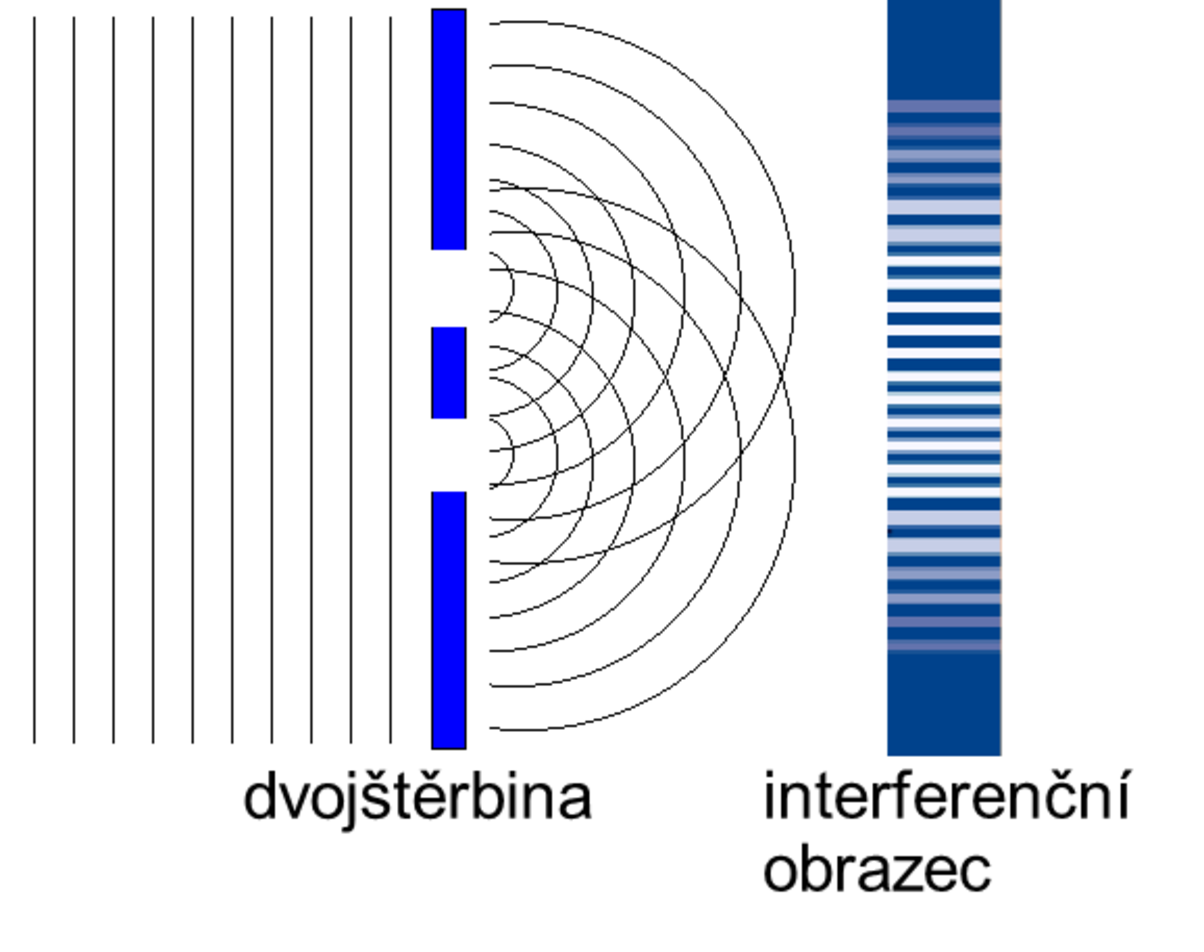
\includegraphics[scale=0.3]{interference.pdf}
\caption[Interference vlnění]{Interference vlnění na dvojštěrbině. Do každého bodu na stínítku dopadá světlo z~obou štěrbin, dochází k~interferenci a na stínítku vznikají světlé a tmavé proužky, tzv. interferenční obrazec.}
\label{obr:Interference}
\end{figure}

Bude užitečné si na začátek zopakovat některé veličiny, které charakterizují vlnění (viz obrázek~\ref{obr:Vlna}).
Vlna je určena velikostí nějaké veličiny (například výšky vodní hladiny či intenzity elektrického pole) měnící se v~prostoru a v~čase, označme si tuto veličinu $A(x,t)$. 
\begin{figure} [ht]
\centering
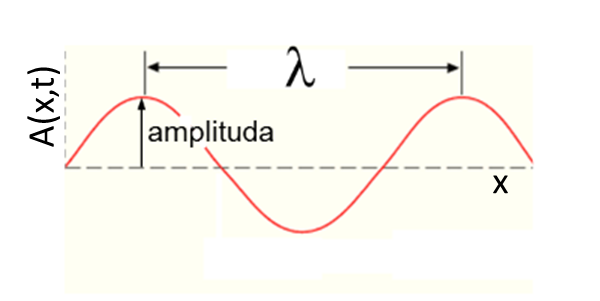
\includegraphics[scale=0.7]{vlna.pdf}
\caption[Znázornění vlny]{Schematické  znázornění vlny.}
\label{obr:Vlna}
\end{figure}

V~nejjednodušším případě se bude vlna šířit harmonicky ve směru osy $x$
\begin{equation}
A(x, t) = A_0 \sin2\pi \left ( \frac{x}{\lambda}-\frac{t}{T} \right) \mbox{,}
\label{rov:Vlna}
\end{equation}
kde $\lambda$ je tzv. \textbf{vlnová délka}, udávající vzdálenost mezi dvěma maximy vlny pro určitý čas a $T$ je \textbf{perioda}, udávající časový interval mezi dosažením maxima vlny pro určité místo. Reciprokou hodnotu periody $T$ označujeme jako  \textbf{frekvenci} $\nu = \frac{1}{T}$. Mezi vlnovou délkou a frekvencí platí vztah
\begin{equation}
\lambda = \frac{c}{\nu}\mbox{.}
\label{rov:Vlna2}
\end{equation}

\noindent K~popisu vlny se také používá veličina \textbf{vlnočet} $\tilde{\nu}=c\nu$\mbox{.} Ten nám udává, kolik vln se umístí do 1 m.
Často se místo vlnové délky a frekvence setkáváme se zápisem pomocí \textbf{vlnového čísla} $k$ a~\textbf{úhlové frekvence} $\omega$
\begin{equation}
k = \frac{2\pi}{\lambda}\mbox{}
\label{rov:Vlna3}
\end{equation}
\begin{equation}
\omega = 2\pi\nu\mbox{.}
\label{rov:Vlna4}
\end{equation}

\noindent Postupné vlnění ve směru osy $x$ má pak tvar
\begin{equation}
A(x,t)=A_0 \sin(kx - \omega t).
\label{rov:Vlna5}
\end{equation}

\noindent Jak jsme již zmínili výše, patří k~základním rysům vlnění jeho skládání. Představme si nyní, že skládáme 2 vlny o~stejné frekvenci, které směřují proti sobě
\begin{equation}
A(x,t)=A_0[\sin (kx-\omega t)+ \sin (kx+\omega t)]\mbox{.}
\label{rov:Vlna6}
\end{equation}

\noindent S~takovouto situací se setkáváme třeba při rozvlnění struny na kytaře. S~využitím vzorců pro sinus součtu úhlů
\begin{equation}
\sin(\alpha \pm \beta) = \sin \alpha\cos\beta \pm \cos\alpha\sin\beta
\label{rov:Vlna7}
\end{equation}

\noindent získáme úpravou
\begin{equation}
A(x,t)=2A_0\sin kx \cos \omega t = A'(x)\cos \omega t.
\label{rov:Vlna8}
\end{equation}

\noindent Vidíme tak, že v~tomto případě bude tvar vlny stále stejný a celá vlna bude pouze periodicky růst a klesat. Mluvíme o~tzv. stojatém vlnění, které je v~chemii velmi důležité.

Ukazuje se, že každé vlnění je možné popsat tzv. vlnovou rovnicí
\begin{equation}
\frac{\partial ^2A(x,t)}{\partial x^2} = \frac{1}{\nu^2}\frac{\partial^2A(x,t)}{\partial t^2}\mbox{.}
\label{rov:Vlna9}
\end{equation}
Z~matematického hlediska jde o~parciální diferenciální rovnici druhého řádu. Tuto rovnici lze kupříkladu pro popis pohybu struny na kytaře odvodit z~Newtonovy mechaniky, v~případě elektromagnetického záření pak zase z~Maxwellových rovnic. 

\subsection{Experimenty, které změnily svět}

Na konci devatenáctého století se fyzika zdála být skoro dobudována. Objekty světa byly uspokojivě popsány buď Newtonovou mechanikou (částice) či Maxwellovou elektrodynamikou. Velké soubory částic pak zpracovávala statistická fyzika a termodynamika. Ve století dvacátém nicméně došlo k~zásadnímu obratu a mnohé jistoty vzaly za své. Níže zběžně popíšeme některé základní experimenty, které lidstvo přivedly od světa klasického do světa kvantového. Tyto experimenty z~různých pohledů ukazovaly na dva základní rysy kvantové mechaniky (a) kvantování energie, (b) vlnově-částicový dualismus.

\subsubsection{Záření absolutně černého tělesa}

Absolutně černým tělesem máme na mysli objekt, který pohltí veškeré dopadající záření, žádné záření tedy není odraženo. Může být realizováno třeba dutinou s~malým otvorem: světlo mnohokráte narazí na stěny nádoby, takže pravděpodobnost, že by odražené světlo vylétlo štěrbinou zase ven, je mizivá. Černé těleso ale zároveň musí energii vyzařovat, jinak by se v~něm hromadila. Badatele zajímalo, jakým způsobem intenzita vyzářeného světla závisí na jeho frekvenci. Experimentálně bylo zjištěno, že hustota záření pro malé frekvence je velmi malá a roste se zvyšující se frekvencí. V~závislosti na teplotě pak dosahuje svého maxima a posléze zase klesá. 

Při teoretickém modelování předpokládáme, že k~vyzařování světla o~určité frekvenci dochází při pohybu dipólu oscilujícího s~určitou frekvencí. Podobně, jako je tomu u~antény vysílače. Tento dipól je uváděn do pohybu díky pohybu nabitých částic. Z~teorie plynul vztah mezi hustotou záření a střední energií oscilátoru při dané teplotě
\begin{equation}
\rho(\nu,T)=\frac{8\pi\nu^2}{c^3}\bar{E}_{osc}\mbox{.}
\label{rov:Cerneteleso1}
\end{equation}
V~klasické mechanice ale platí, že střední energie každého harmonického oscilátoru je nezávislá na frekvenci a rovna $kT$. To by ale znamenalo, že vyzářená energie poroste se čtvercem frekvence! To je sice pravda pro malé frekvence, ale předpověď naprosto selhává pro frekvence vysoké. Vždyť by to znamenalo, že rozžhavený kámen by měl být intenzivním zdrojem rentgenového záření. 

Max Planck přišel s~myšlenkou, že souladu s~experimentem můžeme dosáhnout za předpokladu, že elektromagnetický oscilátor\footnote{ Elektromagnetický oscilátor si můžeme představit jako kladný a záporný náboj spojený pružinkou.} nemůže nabývat libovolných hodnot, nýbrž pouze hodnot
\begin{equation}
E=nh\nu\mbox{,}
\label{rov:Cerneteleso2}
\end{equation}

\noindent kde $h$ je tzv. Planckova konstanta a $n$ je celé číslo. Záření pak může být předáváno pouze po minimálních balíčcích $h\nu$, což je nejmenší rozdíl energie mezi dvěma hladinami oscilátoru. Při konečné teplotě je střední hodnota energie oscilátoru rovna
\begin{equation}
\bar{E}_{osc}=\frac{h\nu}{e^{\frac{h\nu}{kT}}-1}\mbox{}
\label{rov:Cerneteleso3}
\end{equation}
a po dosazení do vztahu \ref{rov:Cerneteleso1} pak získáme
\begin{equation}
\boxed{\rho(\nu,T) = \frac{8\pi h\nu^3}{c^3}\frac{1}{e^{\frac{h\nu}{kT}}-1}\mbox{.}}
\label{rov:Cerneteleso4}
\end{equation}
Tento vztah báječným způsobem souhlasil s~experimentem, pokud za hodnotu konstanty $h$ dosadíme číslo 6,626$\cdot10^{-34}$ J$\cdot$s. Je třeba ale vidět, že souladu s~experimentem bylo dosaženo za použití v~té době dosti bláznivých předpokladů. Předně předpokládáme, že pohyb částic je omezen jen na určité hodnoty energie, je kvantován. Za druhé, předpokládáme, že světlo je předáváno do okolí ve formě jakýchsi dále nedělitelných balíčků energie. Není proto nijak podivné, že Planck celou věc nebral příliš vážně. Planckovu představu ale tvůrčím způsobem využil Albert Einstein ve své teorii fotoelektrického jevu, díky které se právem počítá mezi zakladatele kvantové mechaniky.

\subsubsection{Teorie fotoelektrického jevu}
Základní schéma fotoelektrického jevu je zobrazeno na obrázku~\ref{obr:Fotoefekt}. V~elektrickém obvodu měříme elektrický proud přenášený elektrony, které jsou uvolňovány z~ozařovaných kovových destiček. Ze závislosti prošlého fotoelektrického proudu na vloženém napětí můžeme zjistit jednak maximální kinetickou energii vyražených elektronů i jejich celkové množství.

\begin{figure} [ht]
\centering
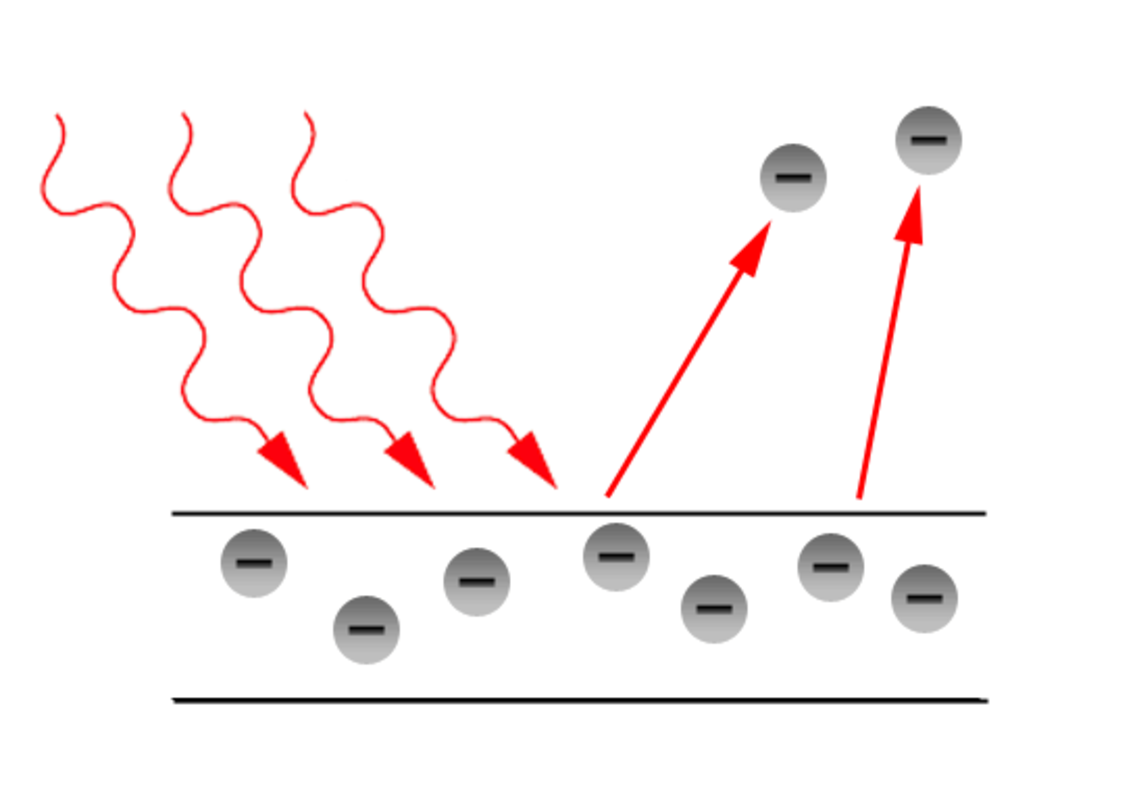
\includegraphics[scale=0.4]{Photoelectric_effect.pdf}
\caption[Fotoelektrický jev]{Schematické znázornění fotoelektrického jevu. Při ozařování kovu ultrafialovými paprsky jsou z~kovu uvolňovány elektrony.}
\label{obr:Fotoefekt}
\end{figure}

Co bychom předpokládali z~hlediska klasické teorie? K~vyražení elektronů by mělo dojít světlem každé vlnové délky, pokud bude mít dostatečnou intenzitu. Ukázalo se však, že k~průchodu fotoelektrického proudu nedocházelo pro frekvence světla nižší než určitá mezní frekvence $\nu_0$, charakteristická pro daný kov. Energie vyražených elektronů pak lineárně rostla s~frekvencí.
Albert Einstein tyto výsledky interpretoval velmi odvážně. Konstatoval, že světlo představuje proud částic o~energii $h\nu$ a vyražení elektronu si pak představoval jako srážkový děj mezi touto světelnou částicí a elektronem. Hypotéza musela působit velmi podivně, vždyť Newtonův pohled na světlo jako na proud částic byl již dávno opuštěn a Maxwellova elektrodynamika měla za sebou lecjaký úspěch. Pro závislost kinetické energie elektronů na frekvenci záření by měla platit rovnice
\begin{equation}
E_{kin} = h\nu - \phi\mbox{,}
\label{rov:Fotojev1}
\end{equation}

\noindent kde $\phi = h\nu_0$ se nazývá výstupní práce. 

Jestliže nafitujeme hodnotu experimentálních dat na rovnici \ref{rov:Fotojev1}, získáme hodnotu $h= 6,626\cdot10^{-34}$ J$\cdot$s. Einsteinův balíček energie je charakterizován úplně stejně jako Planckův balíček energie! Einstein šel ve svých úvahách ještě dále. Je-li podle něj světlo částicí, měla by tato částice (později nazvaná foton) také nějakou hybnost. Jelikož se ale pohybuje rychlostí světla, měla by tato hybnost být dána již relativistickým výrazem
\begin{equation}
p = mv = \frac{m_0 v}{\sqrt{1-\frac{v^2}{c^2}}}\mbox{,}
\label{rov:Fotojev2}
\end{equation}
kde $m_0$ je klidová hmotnost fotonu. Výraz ve jmenovateli je nulový, takže aby hybnost byla rozumné číslo, musí mít foton nutně nulovou klidovou hmotnost. Upravme nyní výraz pro relativistickou hybnost
\begin{equation}
p^2c^2 = \frac{m_0^2v^2c^2}{1-\frac{v^2}{c^2}} = \frac{m_0^2 c^4 [\frac{v^2}{c^2}-1]}{1-\frac{v^2}{c^2}} + \frac{m_0^2 c^4}{1-\frac{v^2}{c^2}} = -m_0^2 c^4 + m^2c^4\mbox{,}
\label{Fotojev3}
\end{equation}
z~čehož
\begin{equation}
E^2 = p^2c^2+ m_0^2c^4\mbox{.}
\label{Fotojev4}
\end{equation}

\noindent Jelikož ale pro foton platí $m_0$ = 0, tak také
\begin{equation}
E=pc\mbox{.}
\label{rov:Fotojev5}
\end{equation}

\noindent S~použitím Planckova vztahu $E = h\nu = \frac{hc}{\lambda}$ dostáváme
\begin{equation}
\boxed{\lambda = \frac{h}{p}\mbox{.}}
\label{rov:Fotojev6}
\end{equation}

\begin{priklad}
\textbf{Zadání:} Kolik fotonů o vlnové délce $396{,}96$~nm zastaví atom vápníku $^{40}$Ca s relativní atomovou hmotností $A_r = 39{,}96$ vypařovaný z kovového vápníku v pícce o teplotě $600\,^{\circ}$C?\\[0.1cm]
\textbf{Řešení:} Atomy vápníku v pícce mají kinetickou energii danou vztahem
\begin{displaymath}
E = \frac{3}{2} kT = 1{,}81 \cdot 10^{-20} \mbox{ J}.
\end{displaymath}
Hybnost je dána jako
\begin{displaymath}
p = \sqrt{2 m E} = 4{,}90 \cdot 10^{-23} \mbox{ kg\cdot m\cdot s}^{-1},
\end{displaymath}
z čehož snadno dopočítáme střední kvadratickou rychlost
\begin{displaymath}
v = \frac{p}/{m} = 738 \mbox{ m\cdot s}^{-1}.
\end{displaymath}
Atom vápníku můžeme zářením ionizovat, vzniklý ion uvěznit v iontové pasti a v ní ho bombardovat zářením. Fotony světla udané vlnové délky mají hybnost
\begin{displaymath}
p_{\mbox{foton}}= \frac{h}/{\lambda} = 1{,}66692 \cdot 10^{-27} \mbox{ kg\cdot m\cdot s}^{-1}.
\end{displaymath}
Při pohlcení jednoho fotonu dojde tedy pouze k docela malé změně rychlosti
\begin{displaymath}
\Delta v = \frac{p_{\mbox{foton}}}/{m} = 2{,}515 \cdot 10^{-2} \mbox{ m\cdot s}^{-1}.
\end{displaymath}
Počet fotonů $x$ nutných k zastavení atomu vápníku pak zjistíme z rovnice $v - x \Delta v =0$. Dosazením dojdeme k hodnotě asi $3 \cdot 10^4$ fotonů, aby se atom vápníku zastavil.
\end{priklad}

\subsubsection{Spektrum atomu vodíku}

V~roce 1897 objevil Joseph John Thompson elektron a v~roce 1911 pak Ernest Rutherford objevil atomové jádro. Nebylo pak těžké si představit atom jako planetární systém, kde okolo těžkého, nabitého jádra obíhá lehký elektron. Takováto představa má ale ve skutečnosti řadu potíží. Předně není vůbec jasné, proč by takovýto atom měl být stabilní. Nabitá částice by dle klasické teorie měla velmi rychle ztrácet svou energii ve formě záření. Rozžhavené atomy navíc vyzařují světlo jen zcela určitých vlnových délek, tj. atomy mají čárové emisní spektrum (viz obrázek~\ref{obr:spectrumH}). 
\begin{figure} [ht]
\centering
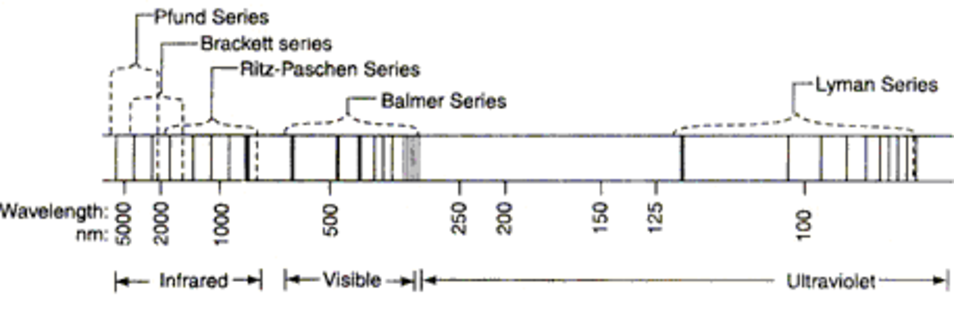
\includegraphics[scale=1]{spectrumH.pdf}
\caption[Emisní spektrum vodíku]{Čárové emisní spektrum atomu vodíku.}
\label{obr:spectrumH}
\end{figure}

Spektrum atomu vodíku představuje řada čar, které je možné sdružit do určitých sérií (Lymanova, Balmerova, Paschenova...). Experimentálně se ukázalo, že vlnočet těchto čar je možné vyjádřit vztahem
\begin{equation}
\tilde{\nu} = 10973731\left( \frac{1}{n_1^2} - \frac{1}{n_2^2}\right ) \mathrm{cm} ^{-1}\mbox{.}
\label{rov:Spektrumvodiku1}
\end{equation}
Niels Bohr dokázal tento vztah v~roce 1913 dát do souvislosti s~planetárním modelem atomu. Předpokládal, že se elektron pohybuje po kruhové dráze, na které musí být odstředivá síla rotující částice kompenzována přitažlivou silou elektrostatickou
\begin{equation}
\frac{m_{e}v^2}{r} = \frac{1}{4\pi \epsilon_0}\frac{Ze^2}{r^2}\mbox{.}
\label{rov:Spektrumvodiku2}
\end{equation}

\noindent Nyní ale máme nekonečné množství stavů, po kterých se částice mohou pohybovat - podle toho, jakou zvolíme rychlost, musíme zvolit také příslušný poloměr. Bohr ale navíc předpokládal, že moment hybnosti může nabývat pouze hodnot celistvých násobků konstanty $\hbar=\frac{h}{2\pi}$
\begin{equation}
m_{e}vr = \hbar n \mbox{.}
\label{rov:Spektrumvodiku3}
\end{equation}
\noindent Proč ho něco takového napadlo? Aby to vyšlo! Z~podmínky \ref{rov:Spektrumvodiku3} vyjádříme rychlost $v$ jako funkci $r$ a dosadíme do podmínky \ref{rov:Spektrumvodiku2}. Získáme vztah
\begin{equation}
r = \frac{4\pi\epsilon_0\hbar^2}{Zm_e e^2}n^2
\label{rov:Spektrumvodiku4}
\end{equation}

\noindent a pro rychlost
\begin{equation}
v = \frac{Ze^2}{4\pi\epsilon_0\hbar}\frac{1}{n}\mbox{.}
\label{rov:Spektrumvodiku5}
\end{equation}

\noindent Po dosazení do vztahu pro energii dostaneme
\begin{equation}
\boxed{E = \frac{1}{2}m_e v^2 - \frac{Ze^2}{4\pi\epsilon_0r} = - \frac{Z^2m_e e^4}{8 \epsilon_0^2\hbar^2}\frac{1}{n^2} = -\frac{13,6 Z^2}{n^2} \mbox{ [eV]}\mbox{.}}
\label{Spektrumvodiku6}
\end{equation}

\noindent Poloměr, rychlost i energie jsou tedy kvantovány. K~přechodu mezi dvěma elektronovými stavy může dojít pouze tehdy, jestliže rozdíl energií počátečního a konečného stavu je roven energii fotonu
\begin{equation}
E_2-E_1 = h\nu,
\label{rov:Spektrumvodiku7}
\end{equation}
tedy
\begin{equation}
\frac{Z^2m_e e^4}{8\epsilon_0^2h^2}\left[ \frac{1}{n_1^2} - \frac{1}{n_2^2} \right ] = h\nu = hc\tilde{\nu}.
\label{rov:Spektrumvodiku8}
\end{equation}

\noindent Pro vlnočet fotonu tak dostaneme
\begin{equation}
\tilde{\nu} = \frac{Z^2m_e e^4}{8\epsilon_0^2 h^3c}\left[ \frac{1}{n_1^2} - \frac{1}{n_2^2} \right ] = 10973731 \left[ \frac{1}{n_1^2} - \frac{1}{n_2^2} \right ].
\label{rov:Spektrumvodiku9}
\end{equation}

\noindent Což je přesně experimentálně pozorovaný vztah! Zdá se tedy, že kvantována není pouze energie, ale také moment hybnosti částice. Kvantování jako by bylo obecným rysem světa molekul. 

\subsection{Dualismus vln a částic}

Einstein svou analýzou fotoelektrického jevu ukázal, že i objekt tak nepochybně vlnový jakým je světlo se za jistých okolností může chovat jako částice. Tato skutečnost je vyjádřena v~rovnicích \ref{rov:Fotojev5} a \ref{rov:Fotojev6}. V~roce 1924 přišel Louis de Broglie s~myšlenkou, že vztah \ref{rov:Fotojev6} se dá číst také opačně: každá hmotná částice s~hybností $mv$ je charakterizována vlnovou délkou $\lambda$ dle vztahu
\begin{equation}
\boxed{\lambda = \frac{h}{mv}\mbox{,}}
\label{rov:Dualismus1}
\end{equation}
\noindent což je tzv. de Broglieův vztah. Sám de Broglie asi příliš netušil, o~jakou vlnu by mělo jít. Nicméně jeho vztah sehrál v~dalším vývoji kvantové teorie zásadní roli. 

De Broglieův vztah umožňuje také interpretovat Bohrovu kvantovou podmínku \ref{rov:Spektrumvodiku3}. Elektron kolem atomového jádra si pak můžeme představit jako stojaté vlnění, kdy na obvod kruhu je třeba vměstnat celistvý násobek de Broglievých vlnových délek
\begin{equation}
2\pi r = n \frac{h}{m_e v}\mbox{,}
\label{Dualismus2}
\end{equation}
tedy
\begin{equation}
m_e vr = \frac{h}{2\pi}n = \hbar n \mbox{.}
\label{Dualismus3}
\end{equation}

Pro objasnění De Brogliova vztahu si vypůjčíme analogii z~optiky, kde je znám Youngův experiment. Mějme dvojici paralelních štěrbin (dvojštěrbinu), na které dopadá monochromatické záření. Záření prochází dvojštěrbinou a  dopadá na stínítko. Výsledkem našeho pozorování bude interferenční obrazec střídajících se světlých a tmavých proužků, které po řadě odpovídají maximům a minimům intenzity dopadajícího světla. Pozorujeme tzv. interferenční obrazec. Maxima odpovídají konstruktivní interferenci, minima naopak interferenci destruktivní. Vysvětlení pozorovaného je následující. Světlo se prostorem šíří jako vlna a jako taková vyplňuje celý dostupný prostor. A~tak nás nepřekvapí, že jedna vlna projde v~jeden okamžik oběma štěrbinami zároveň. Proto je vlna procházející jednou štěrbinou ovlivněna vlnou z~druhé štěrbiny a naopak. Vycházející paprsky spolu interagují, skládají se, což je podstatou pozorované interference.

Proveďme teď stejný experiment jen s~tím rozdílem, že na dvojštěrbinu bude dopadat tok klasických částic. Protože částice je podle klasické mechaniky lokální objekt, zdá se být samozřejmé, že v~daný okamžik může částice projít jen jednou štěrbinou, nikoliv oběma štěrbinami zároveň. Z~klasické mechaniky pak pro intenzitu dopadajících částic vyplývá, že intenzita v~daném bodě stínítka je součtem intenzit, které bychom dostali při otevření pouze první nebo druhé štěrbiny
\begin{equation}
I_{12} = I_1 + I_2 \mbox{.}
\label{rov:IntenzitaKlasickeCastice}
\end{equation}
Rovnice (\ref{rov:IntenzitaKlasickeCastice}) vyjadřuje skutečnost, že přítomnost jedné štěrbiny nijak neovlivňuje to, jakým způsobem částice procházejí druhou štěrbinou.

V~případě světla (Youngův experiment) je situace složitější, protože jak víme, dochází k~interferenci. Tu lze popsat tak, že v~daném bodě na stínítku  se sčítají intenzity (v~případě světla) elektrického pole od obou štěrbin
\begin{equation}
\mathbf{E}_{12} = \mathbf{E}_1 + \mathbf{E}_2 \mbox{.}
\label{rov:IntenzitaSvetla-E}
\end{equation}
Intenzita světla je úměrná kvadrátu velikosti odpovídající intenzity pole, proto v~případě světla dostaneme namísto rovnice (\ref{rov:IntenzitaKlasickeCastice})
\begin{equation}
I_{12} \not = I_1 + I_2 \mbox{.}
\label{rov:IntenzitaSvetla-I}
\end{equation}
Nerovnost ve výrazu (\ref{rov:IntenzitaSvetla-I}) je důsledkem interference světelných paprsků. Světlo v~tomto případě reprezentujeme jako vlnu, takže přítomnost jedné štěrbiny ovlivní průchod světla druhou štěrbinou. Výsledkem je existence interferenčního členu, který způsobí například to, že při otevření obou štěrbin může být intenzita v~daném místě nižší než při otevření jen jedné štěrbiny.

Experiment ještě dále pozměňme. Snižujme intenzitu dopadajícího světla natolik, až proti stínítku bude v~jeden okamžik dopadat vždy jen jeden foton (kvantum elektromagnetického záření). Při dopadu fotonu na stínítko dojde k~ozáření jen jednoho bodu, podobně jako tomu je v~případě klasických částic, kde každá může dopadnout jen na jediné místo na stínítku. Ovšem necháme-li experiment probíhat dostatečně dlouho, začne se z~jednotlivých bodů na stínítku vytvářen stejný interferenční obrazec, jaký bychom dostali v~případě dopadajících světelných vln, analogicky jako v~případě Youngově experimentu. Toto chování nemůžeme vysvětlit jinak, než že i jeden jediný foton je ovlivňován existencí druhé štěrbiny, stejně jako monochromatická vlna.

Podobně jako fotony můžeme nechat na stínítko dopadat tok jiných elementárních částic, například neutronů či elektronů. Výsledek bude totožný tomu, který jsme dostali při experimentu s~fotony. Pozorované interferenční chování částic nemůžeme vysvětlit pomocí teoretického aparátu klasické fyziky. Podle klasické fyziky projde-li částice jednou štěrbinou, nemá na ni přítomnost druhé štěrbiny žádný vliv. Ovšem pozorované interferenční chování částic je experimentálním faktem, který nemůžeme přehlížet. Elegantním řešením je připustit, že částice mají obdobný vlnový charakter jako monochromatické záření. Tento závěr jako první vyslovil Louis de Broglie ve své hypotéze o~dualitě částic a vlnění (viz kapitola \ref{kap:historie}).

U~částic tedy můžeme pozorovat kvantově-mechanické interference, které lze popsat tak, že každé částici přiřadíme vlnovou funkci $\psi(x, t)$, která je funkcí prostorových souřadnic a~času. Přidržíme-li se i nadále analogie s~optikou, můžeme hustotu pravděpodobnosti $\rho$ nalezení částice v~daném místě $x$ a čase $t$ vyjádřit jako
\begin{equation}
\rho(x, t) = |\psi(x,t)|^2 \mbox{.}
\label{rov:VlnovaFce-castice}
\end{equation}
Vzhledem k~tomu, že kvadrát vlnové funkce interpretujeme jako pravděpodobnost (viz Bornova pravděpodobnostní interpretace kvantové mechaniky v~kapitole \ref{kap:historie}), musí platit rovnice
\begin{equation}
\int |\psi(x,t)|^2 \,\mathrm{d}x = 1 \mbox{,}
\label{rov:Normalizace}
\end{equation}
která vyjadřuje skutečnost, že částice se musí někde vyskytovat. Rovnice (\ref{rov:Normalizace}) vyjadřuje tzv. normalizační podmínku.

Pokud zavedeme po řadě pro pravděpodobnosti dopadu částice na stínítko při otevřené první nebo druhé štěrbině označení $p_1$ a $p_2$, pak pravděpodobnost dopadu na dané místo stínítka při obou otevřených štěrbinách se nerovná součtu pravděpodobností $p_1$ a $p_2$
\begin{equation}
p_{12} \not = p_1 + p_2 \mbox{,}
\label{rov:Pravdepodobnosti-Stinitko}
\end{equation}
ale pravděpodobnost bude záviset na interferenčním členu. Můžeme dokonce dostat výsledek takový, že $p_{12} = 0$, přestože $p_1 \not =  0$ a $p_2 \not = 0$, což vede k~minimu intenzity na stínítku (analogie s~destruktivní interferencí).

De Brogliův vztah byl v~roce 1928 experimentálně potvrzen experimentem Davissona a~Germera, kteří na krystalu niklu pozorovali difrakci elektronových vln.

\subsection{Pohybové rovnice kvantově-mechanických částic: Schr\"odingerova rovnice}

Bohrova teorie dokázala popsat atom vodíku, dokázala také alespoň naznačit princip vzniků molekul, ale brzy začalo být zřejmé, že teorie má své limity. Ve dvacátých letech se odehrálo mnoho chytrých pokusů spojit klasickou mechaniku s~experimentálním pozorováním kvantování energie, ale průlom přišel až s~vytvořením zcela nové, kvantové mechaniky. Ta se na konci dvacátých let objevila ve dvou formách, Heisenbergově maticové mechanice a Schr\"odingerově vlnové mechanice, i když na první pohled nebylo vůbec zřejmé, že tyto dvě mechaniky mají něco společného. My zde budeme alespoň náznakem sledovat myšlenkový postup Erwina Schr\"odingera.

Na začátku je třeba říci, že kvantová mechanika je založena na postulátech a jako takovou ji nemůžeme odvodit. Můžeme ji pouze uhodnout. To ale neznamená, že bychom neměli žádné indicie. 
Schr\"odinger mohl postupovat asi takto. Řekněme, že nás zajímají stacionární stavy částic, například atomů. Ty budou nejspíše popsány stojatou vlnou
\begin{equation}
\Psi(x,t) = \psi(x)cos(\omega t)\mbox{.}
\label{rov:Pohyboverovnice1}
\end{equation}
Pro všechny vlny platí vlnová rovnice, měla by proto platit i pro vlnu popisující elektron. Tj.
\begin{equation}
\frac{\partial^2\Psi(x,t)}{\partial x^2} = \frac{1}{v^2}\frac{\partial^2\Psi(x,t)}{\partial t^2}\mbox{.}
\label{rov:Pohyboverovnice2}
\end{equation}
\noindent Po dosazení ze vztahu \ref{rov:Pohyboverovnice1}
\begin{equation}
\frac{\dd^2\psi(x)}{\dd x^2} + \frac{\omega^2}{v^2}\psi(x) = 0 \mbox{.}
\label{rov:Pohyboverovnice3}
\end{equation}
\noindent Uvažme nyní, že
\begin{equation}
\omega = 2\pi\nu = \frac{2\pi v}{\lambda}
\label{rov:Pohyboverovnice4}
\end{equation}
\noindent a dosaďme za vlnovou délku z~de Brogliova vztahu $\lambda = \frac{h}{p}$ a za $\frac{p^2}{2m}=E-V$.
Úpravou dostáváme
\begin{equation}
\frac{\dd^2\psi(x)}{\dd x^2} + \frac{8\pi^2 m}{h^2}[E - V(x)]\psi(x) = 0 
\label{rov:Pohyboverovnice5}
\end{equation}

\noindent nebo též
\begin{equation}
\boxed{-\frac{\hbar^2}{2m}\frac{\dd^2\psi(x)}{\dd x^2} + V(x)\psi(x) = E\psi(x) \mbox{.}}
\label{rov:Pohyboverovnice6}
\end{equation}

\noindent Což je tzv. bezčasová Schr\"odingerova rovnice. Kompaktně jí můžeme napsat jako
\begin{equation}
\hat{H}\psi = E\psi\mbox{,}
\label{rov:Pohyboverovnice7}
\end{equation}

\noindent kde symbolem $\hat{H}$ rozumíme operátor
\begin{equation}
\hat{H} = -\frac{\hbar^2}{2m}\frac{\dd^2}{\dd x^2} + V\mbox{.}
\label{rov:Pohyboverovnice8}
\end{equation}

\noindent Jejím řešením jsou možné hodnoty energie a jím příslušející vlnové funkce. Je to poněkud zvláštní rovnice, neboť má dvě neznámé veličiny, $E$ a funkci $\psi$. Zdálo by se tedy, že kupříkladu energii si můžeme zvolit a vlnovou funkci k~ní dopočítat. Obecně to ale neplatí. 

\subsection{Bornova interpretace vlnové funkce}
\label{kap:Bornova interpretace vlnové funkce}

Co to vlastně je ona vlnová funkce?  Můžeme vyjít z~analogie z~optiky. Roli vlnové funkce zde hraje kupříkladu vektor intenzity elektrického pole. Intenzita světla v~určitém bodě je pak dána jako čtverec intenzity elektrického pole.
Vedeni touto analogií, můžeme s~Maxem Bornem interpretovat vlnovou funkci jako amplitudu pravděpodobnosti. Čtverec vlnové funkce bude mít pak význam hustoty pravděpodobnosti nalezení dané částice v~určitém bodě
\begin{equation}
P(x)\dd x = |\Psi (x)|^2\dd x \mbox{.}
\label{rov:Born1}
\end{equation}

\noindent Z~této interpretace pak plyne tzv. normalizační podmínka
\begin{equation}
\int |\Psi(x)|^2 \dd x = 1\mbox{,}
\label{rov:Born2}
\end{equation}

\noindent která říká, že částice musí být někde v~prostoru. Tato podmínka vlastně představuje další rovnici, kterou musíme dodat ke Schr\"odingerově rovnici. Na vlnovou funkci pak s~ohledem na obě rovnice klademe několik podmínek:
\begin{itemize}
\item Vlnová funkce musí být kvadraticky integrovatelná
\item Vlnová funkce musí být spojitá
\item Vlnová funkce musí mít spojité první derivace
\end{itemize}

\begin{priklad}
\textbf{Zadání:} Které z~funkcí a) - f) mohou být vlnovými funkcemi?

\begin{center}
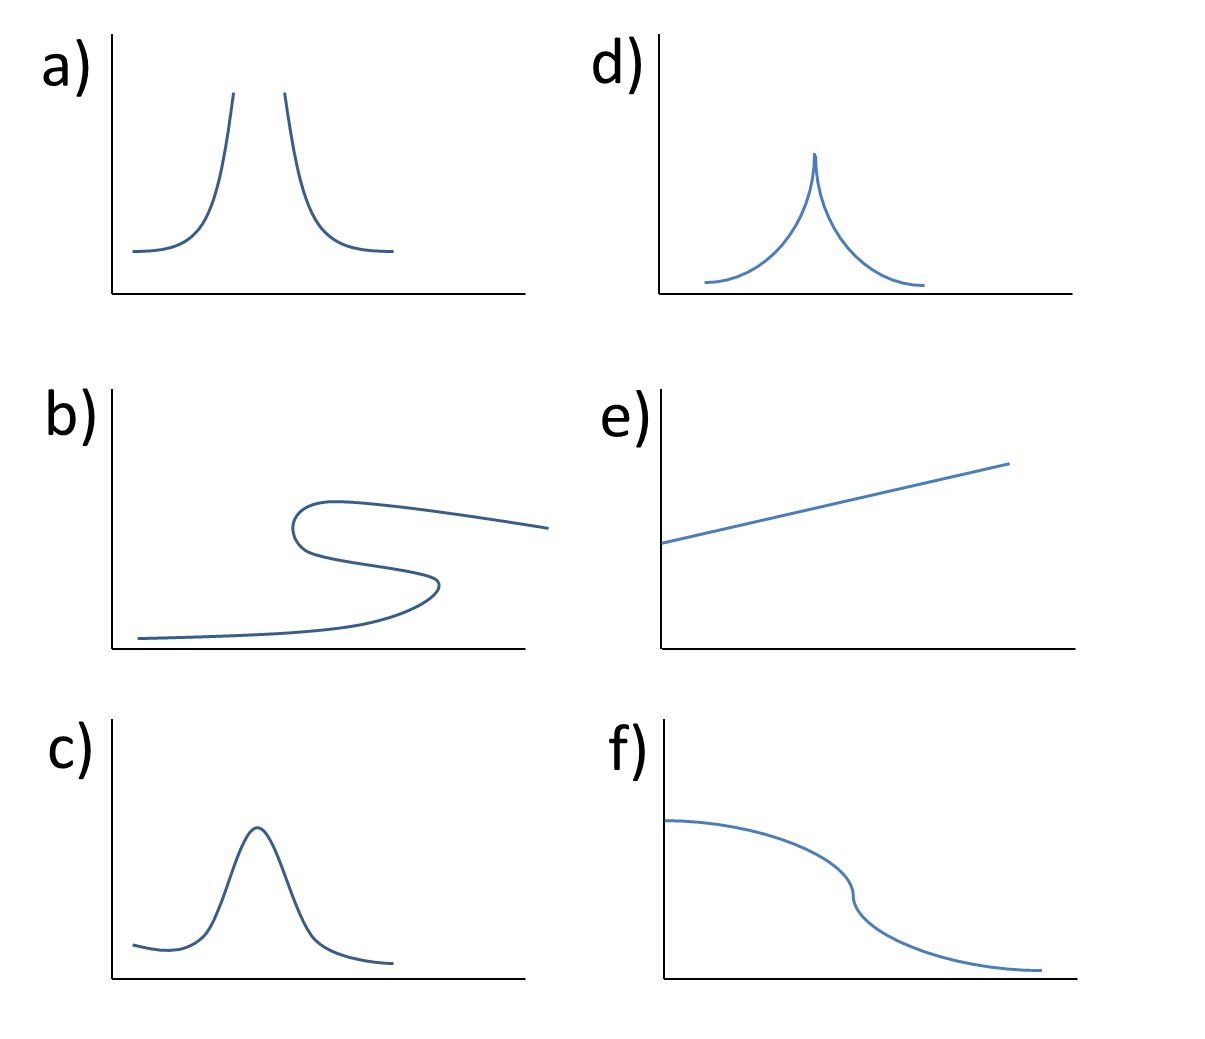
\includegraphics[scale=0.4]{funkce.pdf}

\end{center}

\textbf{Řešení:} a) ne, není spojitá b) ne, není funkce c) ano d) ne, nemá spojitou první derivaci e) ne, není kvadraticky integrovatelná f) ano.
\end{priklad}

\subsection{Časově-závislá Schr\"odingerova rovnice}
Výše jsme si navodili časově-nezávislou Schr\"odingerovu rovnici, jejímž řešením získáme možné energie, se kterými se částice může pohybovat. Časově-nezávislá Schr\"odingerova rovnice se dá odvodit z~časově-závislé Schr\"odingerovy rovnice
\begin{equation}
\boxed{i\hbar \frac{\partial\Psi}{\partial t} = \hat{H}\Psi \mbox{.}}
\label{rov:Casovachr1}
\end{equation}

\noindent Tato rovnice nám ukazuje vývoj stavu v~čase. Známe-li vlnovou funkci v~nějakém čase $t$, integrací Schr\"odingerovy rovnice získáme vlnovou funkci v~libovolném čase příštím (a minulém). V~chemii tato rovnice hraje roli kupříkladu ve spektroskopii: máme molekulu v~základním stavu a zajímá nás, v~jakém stavu se bude molekula nacházet po \uv{zapnutí} vnějšího časově-závislého elektromagnetického pole. V~dalším výkladu se ovšem s~časově-závislou Schr\"odingerovou rovnicí již příliš setkávat nebudeme. 

\subsection{Relace neurčitosti}

Měření veličin v~kvantové mechanice má určitá specifika. Existují skupiny veličin, tzv. komplementární veličiny, které nelze měřit zároveň s~libovolnou přesností. K~těm patří například dvojice poloha-hybnost či $x$-ová a $y$-ová souřadnice momentu hybnosti. Ze Schr\"odingerovy rovnice se dá dokázat, že
\begin{equation}
\boxed{\Delta x \Delta p \geq \frac{\hbar}{2}\mbox{,}}
\label{rov:Neurcitost1}
\end{equation}

\noindent kde $\Delta x$ je neurčitost polohy a $\Delta p$ je neurčitost hybnosti. Čím přesněji měříme polohu, tím méně přesnou máme hybnost. Důsledkem je mimo jiné neexistence pojmu trajektorie částice v~kvantové mechanice a nerozlišitelnost identických částic. Analogický vztah je mezi neurčitostí energie a času
\begin{equation}
\boxed{\Delta t \Delta E \geq \frac{\hbar}{2}\mbox{,}}
\label{rov:Neurcitostě}
\end{equation}

\noindent což má své důsledky například ve spektroskopii. V~daném časovém intervalu $\Delta t$ jsme schopni změřit energii pouze s~přesností $\Delta E$. Pokud bychom měřili energii přesněji, museli bychom zvětšit $\Delta t$, což může být doba experimentu nebo doba, po kterou daný stav existuje. Pokud nás tedy zajímají procesy s~velmi krátkou dobou života, musíme počítat s~velkou neurčitostí energie.  

Relace neurčitosti se dají \uv{odvodit} také z~částicové povahy světla. Pokud chceme měřit přesně polohu částice, můžeme jí pozorovat pomocí světla. Nepřesnost měření bude dána vlnovou délkou světla $\lambda$, její snižování tak povede ke zvětšování přesnosti. Interakce světla s~pozorovaným objektem na druhou stranu povede k~předání hybnosti o~řádové hodnotě
\begin{equation}
\Delta p = \frac{h}{\lambda}.
\label{rov:Neurcitost2}
\end{equation}

\noindent Což povede k~neurčitosti měření hybnosti. Zároveň $\Delta x \approx \lambda $. Vynásobením pak získáme vztah
\begin{equation}
\Delta x \Delta p \approx h \mbox{,}
\label{rov:Neurcitost3}
\end{equation}

\noindent který je v~souladu s~obecnějším vztahem \ref{rov:Neurcitost1}.
 
\begin{priklad}
\textbf{Zadání:} Elektronový svazek má rychlost $1000 \pm 0{,}01 \mbox{ m}\cdot \mbox{s}^{-1}$. Jak přesně můžeme určit v~daném okamžiku polohu elektronu?

\textbf{Řešení:} Neurčitost hybnosti elektronu je dána vztahem
\begin{displaymath}
\Delta p_x = (0{,}01)(9{,}11 \cdot 10^{-31}) = 9{,}11\cdot 10^{-33} \mbox{ kg\cdot m\cdot s}^{-1}
\end{displaymath}
Neurčitost polohy je potom dána vztahem
\begin{displaymath}
x\geq\frac{\hbar}{2\cdot 9{,}11\cdot 10^{-33}} = 0{,}0058 \mbox{ m} = 0{,}58 \mbox{ cm}.
\end{displaymath}
\end{priklad}

\begin{table}
\centering
\caption{Klasická mechanika vs Kvantová mechanika}
\renewcommand{\arraystretch}{1.8}
\begin{tabular}{p{7cm}cc}
\toprule
 & klas. mech. & kvant. mech\\
\midrule
Stav &$r, p$  & $\Psi(x,t)$ \\
Pohybové rovnice & $m\frac{\dd ^2 r}{\dd t^2} = \nabla V$ & $ i\hbar\frac{\partial \Psi}{\partial t} = \hat{H}\Psi$\\
Časově-nezávislé rovnice & $\frac{mv^2}{r} = F $ & $\hat{H}\psi = E\psi$ \\
Relace neurčitosti & - & $\Delta x \Delta p \geqq \frac{\hbar}{2} \mbox {          atp. }$ \\
\bottomrule
\end{tabular}
\end{table}


\subsection{Postuláty kvantové mechaniky}

Kvantová mechanika je stavěna axiomaticky, je tedy založena (podobně jako termodynamika) na sadě tvrzení, které není možné dokázat. Z~nich se poté tvoří celá stavba kvantové mechaniky. Pokud by postuláty vedly k~důsledkům, jež by byly v~rozporu se zkušeností, bylo by třeba se postulátů vzdát.

{\bf 1. postulát}: Stav kvantově-mechanické soustavy je plně určen vlnovou funkcí $\Psi(x,t_0)$. Pravděpodobnost nalezení částice v~elementu d$x$ kolem $x_0$ je  $|\Psi(x_0,t)|^2\dd x$

\begin{itemize}
\item \textit{Poznámka 1}: Z~postulátu vyplývá normalizační podmínka \ref{rov:Born2}.
\item \textit{Poznámka 2}: Na vlnovou podmínku jsou kladeny podmínky viz podkapitola \ref{kap:Bornova interpretace vlnové funkce}.
\end{itemize}

{\bf 2. postulát}: Pro každou měřitelnou veličinu v~klasické mechanice (poloha, hybnost) existuje korespondující operátor.

{\bf 3. postulát}: V~experimentu je možné změřit pouze hodnoty, které jsou vlastními hodnotami daného operátoru.
\begin{itemize}
\item \textit{Poznámka 1}: Operátory jsou hermitovské. Pak totiž budou vlastní čísla reálná, což bychom u~měřené veličiny očekávali.
\item \textit{Poznámka 2}: Spolu se Schr\"odingerem jsme vyspekulovali operátor celkové energie
\begin{equation}
\hat{H} = - \frac{\hbar^2}{2m}\frac{\dd ^2}{\dd x^2} + V \mbox{.}
\label{rov:Postulaty1}
\end{equation}

\noindent Porovnáním s~klasickým výrazem pro energii

\begin{equation}
E = \frac{p^2}{2m} + V
\label{rov:Postulaty2}
\end{equation}

\noindent můžeme usuzovat, že operátor pro polohu bude poloha a operátor hybnosti

\begin{equation}
\boxed{\hat{p} \rightarrow - i\hbar \frac{\partial}{\partial x}}
\label{rov:Postulaty3}
\end{equation}
\begin{equation}
\boxed{\hat{x} \rightarrow   x}
\label{rov:Postulaty4}
\end{equation}
\end{itemize}

{\bf 4. postulát}: Jestliže se částice nachází ve stavu popsaném vlnovou funkcí $\Psi(x,t)$, pak sada identických měření veličiny $A$ povede ke střední hodnotě
\begin{equation}
\boxed{\langle A \rangle = \frac{\int \Psi^*\hat{A}\Psi \dd x}{\int \Psi^*\Psi \dd x}\mbox{.}}
\label{rov:Postulaty5}
\end{equation}
\begin{itemize}
\item \textit{Poznámka 1}: Pro normalizovanou vlnovou funkci $\psi$ je
\begin{equation}
\braket{A} = \int \psi^{\ast} \hat{A} \psi \mathrm{d} x.
\end{equation}
\end{itemize}

{\bf 5. postulát}: Vývoj kvantově-mechanického stavu se řídí časově-závislou Schr\"odingerovou rovnicí

\begin{equation}
\boxed{i\hbar \frac{\partial \Psi}{\partial t} = \hat{H}\Psi \mbox{.}}
\label{rov:Postulaty6}
\end{equation}

\subsection{Kvantová mechanika pro systém o~více částicích}

Doposud jsme se zabývali pouze jednou částicí pohybující se ve směru osy $x$. Schr\"odingerova rovnice pak má tvar
\begin{equation}
\hat{H}\psi = E\psi \mbox{,}
\label{rov:Vicecastic1}
\end{equation}
kde
\begin{equation}
\hat{H} = -\frac{\hbar^2}{2m}\frac{\dd ^2}{\dd x^2} + V{.}
\label{rov:Vicecastic2}
\end{equation}

\noindent Zobecnění na tři dimenze je triviální
\begin{equation}
\hat{H} = -\frac{\hbar^2}{2m}\left( \frac{\partial^2}{\partial x^2} + \frac{\partial^2}{\partial y^2} + \frac{\partial^2}{\partial z^2} \right ) + V \mbox{.}
\label{rov:Vicecastic3}
\end{equation}

\noindent Zobecnění pro více částic pak v~podobném duchu
\begin{equation}
\hat{H} = \hat{T_1} + \hat{T_2} + \hat{T_3} + .... + \hat{T_N} + V = -\frac{\hbar^2}{2m}\Delta_1 - \frac{\hbar^2}{2m}\Delta_2 - \frac{\hbar^2}{2m}\Delta_3 - .... - \frac{\hbar^2}{2m}\Delta_N + V \mbox{,}
\label{rov:Vicecastic4}
\end{equation}
kde
\begin{equation}
\Delta_i = \frac{\partial^2}{\partial x_i^2} + \frac{\partial^2}{\partial y_i^2} + \frac{\partial^2}{\partial z_i^2}
\label{rov:Vicecastic5}
\end{equation}

\begin{priklad}
\textbf{Zadání:}  Zapište Hamiltonův operátor pro molekulu H$_2^{+}$.

\begin{center}
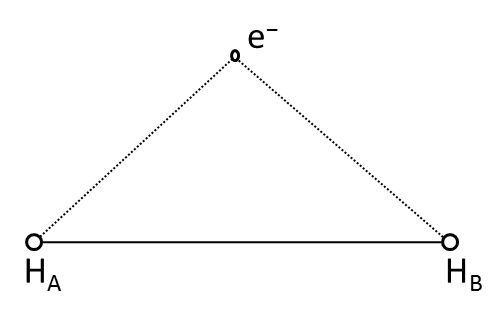
\includegraphics[scale=0.5]{prikladH.pdf}

\end{center}

\textbf{Řešení:}
\begin{equation}
\hat{H} = -\frac{\hbar ^2}{2m_A} \Delta _A - \frac{\hbar^2}{2m_B}\Delta _B -\frac{\hbar^2}{2m_e}\Delta _e + \frac{1}{4\pi \epsilon _0} \left( \frac{e^2}{(\vec{r_A} - \vec{r_B})} - \frac{e^2}{(\vec{r_A} - \vec{r_e})}  - \frac{e^2}{(\vec{r_B} - \vec{r_e})} \right)
\nonumber
\label{rov:Vicecastic6}
\end{equation}

\end{priklad}





